\subsubsection{Generalisation to obstacles not seen in training}
\label{sec:res-general}

\paragraph{Unseen heights.} Real obstacles have arbitrary heights, so the regression was also trained with one height level removed
from the training data (Table~\ref{tab:unseenheight}). Interpolation works: a ridge model that never saw the middle height (H2)
estimates it with a 3.1\,cm mean absolute error and puts 79\,\% of those crossings at the right level (88\,\% when trained on all
heights). Extrapolation is biased toward the trained range: an unseen lowest or highest height is over- or under-estimated by about
half a step (+4.0 and $-5.7$\,cm). The random forest cannot extrapolate at all (an unseen H1 or H3 is off by a full step), and the
generic models are worse throughout. A device for obstacles of any height should therefore be trained on obstacles that span the
heights it will meet, with a model that scales linearly with height.

\begin{table}[htbp]
\centering
\caption{Height in cm when a height level is missing from training (person scaling). Cells: mean absolute error in cm (mean signed
error, + = too high); ``right level'' = the estimate is closest to the person's true nominal height.}
\label{tab:unseenheight}
\begin{adjustbox}{max width=\textwidth}
{\scriptsize
\begin{tabular}{llrrrr}
\toprule
\textbf{model} & \textbf{training} & \textbf{H1 tested} & \textbf{H2 tested} & \textbf{H3 tested} & \textbf{all} \\
\midrule
ridge & all heights trained & 3.0 (+1.4); right level 81\% & 2.6 (+1.0); right level 88\% & 3.8 ($-$2.3); right level 77\% & 3.1 (+0.1); right level 82\% \\
ridge & this height left out & 4.7 (+4.0); right level 50\% & 3.1 (+1.8); right level 79\% & 6.0 ($-$5.7); right level 37\% & 4.6 (+0.2); right level 56\% \\
forest & all heights trained & 1.4 (+1.2); right level 91\% & 2.7 (+1.1); right level 86\% & 3.1 ($-$2.6); right level 79\% & 2.4 ($-$0.0); right level 85\% \\
forest & this height left out & 10.8 (+10.8); right level 0\% & 5.3 (+3.1); right level 42\% & 9.8 ($-$9.8); right level 0\% & 8.6 (+1.6); right level 15\% \\
\bottomrule
\end{tabular}
}
\end{adjustbox}

\end{table}

\paragraph{Unseen width.} Height recognition trained on crossings of one width only and tested on the other width loses about
6.5 points compared with training on the same width with the same amount of data (86.2\,\% vs 92.7\,\%, Table~\ref{tab:unseenwidth}):
although width itself is barely recognisable, the obstacle depth slightly changes how the height shows in the foot motion, so
training data should include obstacles of different depths.

\begin{table}[htbp]
\centering
\caption{Height recognition tested on one width, trained on the same width, the other width only, or both (two foot IMUs, person
scaling, forest vote).}
\label{tab:unseenwidth}
\begin{adjustbox}{max width=\textwidth}
{\footnotesize
\begin{tabular}{lrrr}
\toprule
\textbf{tested on} & \textbf{trained on the same width} & \textbf{trained on the other width only} & \textbf{trained on both widths} \\
\midrule
W1 (5 cm) & 91.2\% & 86.3\% & 94.3\% \\
W2 (15 cm) & 94.0\% & 86.1\% & 90.5\% \\
both widths & 92.7\% & 86.2\% & 92.3\% \\
\bottomrule
\end{tabular}
}
\end{adjustbox}

\end{table}

\subsubsection{What the device model relies on}

For the final two-foot model (person scaling, forest vote, 92.3\,\%), shuffling all features of one foot within each left-out
participant costs 33.4 points (trailing foot) and 24.5 points (leading foot): the model uses both feet
(Table~\ref{tab:importance}). Within a foot, the foot-trajectory summaries matter most (about 6 points each), followed by the
clearance-shape features (about 3) and the foot tilt and angular velocity (about 2); the foot acceleration hardly matters. No single
feature costs more than 2.5 points (Table~\ref{tab:importancetop}): the information is spread over redundant features, the most
useful being how high each foot rises (peak foot height, height at 25\,\% of the trailing swing) and the trailing stance time.

\begin{table}[htbp]
\centering
\begin{minipage}{0.52\textwidth}
\centering
\caption{Permutation importance of feature groups (accuracy drop, mean $\pm$ SD over 10 shuffles).}
\label{tab:importance}
\begin{adjustbox}{max width=\textwidth}
{\footnotesize
\begin{tabular}{lrr}
\toprule
\textbf{shuffled feature group} & \textbf{features} & \textbf{accuracy drop (points)} \\
\midrule
trail foot, all features & 41 & 33.4 $\pm$ 3.4 \\
lead foot, all features & 46 & 24.5 $\pm$ 1.7 \\
trail: foot trajectory summaries & 11 & 6.0 $\pm$ 0.9 \\
lead: foot trajectory summaries & 11 & 5.7 $\pm$ 1.0 \\
trail: clearance shape & 13 & 2.9 $\pm$ 0.8 \\
lead: clearance shape & 13 & 2.9 $\pm$ 1.0 \\
trail: foot tilt and angular velocity & 14 & 2.2 $\pm$ 1.0 \\
lead: foot tilt and angular velocity & 14 & 2.2 $\pm$ 1.0 \\
trail: timing and approach strides & 2 & 1.9 $\pm$ 0.7 \\
lead: timing and approach strides & 7 & 0.7 $\pm$ 0.5 \\
trail: foot acceleration & 3 & 0.7 $\pm$ 0.3 \\
lead: foot acceleration & 3 & 0.2 $\pm$ 0.3 \\
\bottomrule
\end{tabular}
}
\end{adjustbox}

\end{minipage}\hfill
\begin{minipage}{0.44\textwidth}
\centering
\caption{The 12 most important single features.}
\label{tab:importancetop}
\begin{adjustbox}{max width=\textwidth}
{\footnotesize
\begin{tabular}{lr}
\toprule
\textbf{feature} & \textbf{accuracy drop (points)} \\
\midrule
\texttt{trail: trail\_\allowbreak{}zhc\_\allowbreak{}peak\_\allowbreak{}foot\_\allowbreak{}h} & 2.5 $\pm$ 0.7 \\
\texttt{trail: trail\_\allowbreak{}zhc\_\allowbreak{}h\_\allowbreak{}25} & 2.5 $\pm$ 0.8 \\
\texttt{trail: shape\_\allowbreak{}h\_\allowbreak{}peak} & 2.5 $\pm$ 1.0 \\
\texttt{lead: shape\_\allowbreak{}h\_\allowbreak{}peak} & 2.1 $\pm$ 0.9 \\
\texttt{lead: lead\_\allowbreak{}zhc\_\allowbreak{}peak\_\allowbreak{}foot\_\allowbreak{}h} & 2.0 $\pm$ 1.0 \\
\texttt{trail: trail\_\allowbreak{}stance\_\allowbreak{}time} & 2.0 $\pm$ 0.7 \\
\texttt{trail: trail\_\allowbreak{}zhc\_\allowbreak{}h\_\allowbreak{}toeoff} & 2.0 $\pm$ 0.8 \\
\texttt{trail: trail\_\allowbreak{}zhc\_\allowbreak{}h\_\allowbreak{}50} & 1.1 $\pm$ 0.6 \\
\texttt{lead: lead\_\allowbreak{}zhc\_\allowbreak{}h\_\allowbreak{}50} & 0.9 $\pm$ 0.6 \\
\texttt{trail: shape\_\allowbreak{}rise\_\allowbreak{}fall} & 0.9 $\pm$ 0.4 \\
\texttt{lead: cadence} & 0.7 $\pm$ 0.6 \\
\texttt{trail: trail\_\allowbreak{}foot\_\allowbreak{}av\_\allowbreak{}min} & 0.6 $\pm$ 0.3 \\
\bottomrule
\end{tabular}
}
\end{adjustbox}

\end{minipage}
\end{table}

\subsubsection{Statistics for the main comparisons}

\paragraph{Paired differences.} On the same crossings (Table~\ref{tab:paired}), person scaling adds 34.8 points to the two-foot
model (95\,\% CI +22.3 to +46.2), and the 13 clearance-shape features add 10.7 points to a generic model (+4.9 to +16.9). Six IMUs
are not better than two foot IMUs (+1.1, CI $-0.5$ to +3.0), and the trailing foot adds 3.5 points to the leading foot alone (CI
$-1.0$ to +7.2, not significant with ten participants).

\begin{table}[htbp]
\centering
\caption{Paired comparisons on the same crossings (participant bootstrap of the difference).}
\label{tab:paired}
\begin{adjustbox}{max width=\textwidth}
{\footnotesize
\begin{tabular}{p{7.8cm}rrr}
\toprule
\textbf{comparison} & \textbf{A} & \textbf{B} & \textbf{A - B (95\% CI)} \\
\midrule
person scaling vs generic (two foot IMUs, forest) & 92.3\% & 57.5\% & +34.8 (+22.3 to +46.2) \\
two foot IMUs vs all six IMUs (person scaling, forest) & 92.3\% & 91.2\% & +1.1 ($-$0.5 to +3.0) \\
both feet vs leading foot only (person scaling, forest) & 92.3\% & 88.8\% & +3.5 ($-$1.0 to +7.2) \\
13 clearance-shape vs 57 summary features (generic, logistic, leading limb) & 72.8\% & 62.1\% & +10.7 (+4.9 to +16.9) \\
\bottomrule
\end{tabular}
}
\end{adjustbox}

\end{table}

\paragraph{Errors.} The final model recognises 95\,\% of H1, 90\,\% of H2 and 91\,\% of H3 crossings; its errors are almost all
between neighbouring heights (one H3 crossing was called H1; Table~\ref{tab:confusion}).

\paragraph{Can the probabilities be trusted?} The person-scaled forest is \emph{under}-confident (Table~\ref{tab:reliability},
Figure~\ref{fig:validate}): crossings for which it states 55\,\% are right 80\,\% of the time, and from 0.7 upward it is right
96--100\,\% of the time. Its Brier score is 0.18, against 0.51 for the generic model (Table~\ref{tab:brier}). A confidence
threshold is therefore safe for this model: the stated probability understates its reliability.

\begin{table}[htbp]
\centering
\begin{minipage}{0.4\textwidth}
\centering
\caption{Confusion matrix of the final model.}
\label{tab:confusion}
\begin{adjustbox}{max width=\textwidth}
{\footnotesize
\begin{tabular}{lrrrr}
\toprule
\textbf{true \textbackslash{} predicted} & \textbf{H1} & \textbf{H2} & \textbf{H3} & \textbf{correct} \\
\midrule
H1 & 84 & 4 & 0 & 95\% \\
H2 & 0 & 81 & 9 & 90\% \\
H3 & 1 & 6 & 75 & 91\% \\
\bottomrule
\end{tabular}
}
\end{adjustbox}

\end{minipage}\hfill
\begin{minipage}{0.56\textwidth}
\centering
\caption{Brier score and expected calibration error (ECE).}
\label{tab:brier}
\begin{adjustbox}{max width=\textwidth}
{\footnotesize
\begin{tabular}{lrr}
\toprule
\textbf{model} & \textbf{Brier} & \textbf{ECE} \\
\midrule
final (person scaling) & 0.182 & 16.6 points \\
generic (level-walk scaling) & 0.506 & 9.4 points \\
\bottomrule
\end{tabular}
}
\end{adjustbox}

\end{minipage}
\end{table}

\begin{table}[htbp]
\centering
\caption{Reliability: crossings grouped by the stated top-class probability; number, mean stated probability and observed accuracy.}
\label{tab:reliability}
\begin{adjustbox}{max width=\textwidth}
{\footnotesize
\begin{tabular}{lrr}
\toprule
\textbf{stated probability} & \textbf{final: crossings, mean stated, observed} & \textbf{generic: crossings, mean stated, observed} \\
\midrule
0.33--0.50 & 15, 48\%, 67\% & 85, 44\%, 44\% \\
0.50--0.60 & 40, 55\%, 80\% & 53, 54\%, 49\% \\
0.60--0.70 & 30, 65\%, 90\% & 38, 65\%, 32\% \\
0.70--0.80 & 55, 75\%, 96\% & 39, 75\%, 82\% \\
0.80--0.90 & 68, 85\%, 97\% & 39, 84\%, 90\% \\
0.90--1.00 & 52, 94\%, 100\% & 6, 93\%, 100\% \\
\bottomrule
\end{tabular}
}
\end{adjustbox}

\end{table}

\begin{figure}[htbp]
\centering
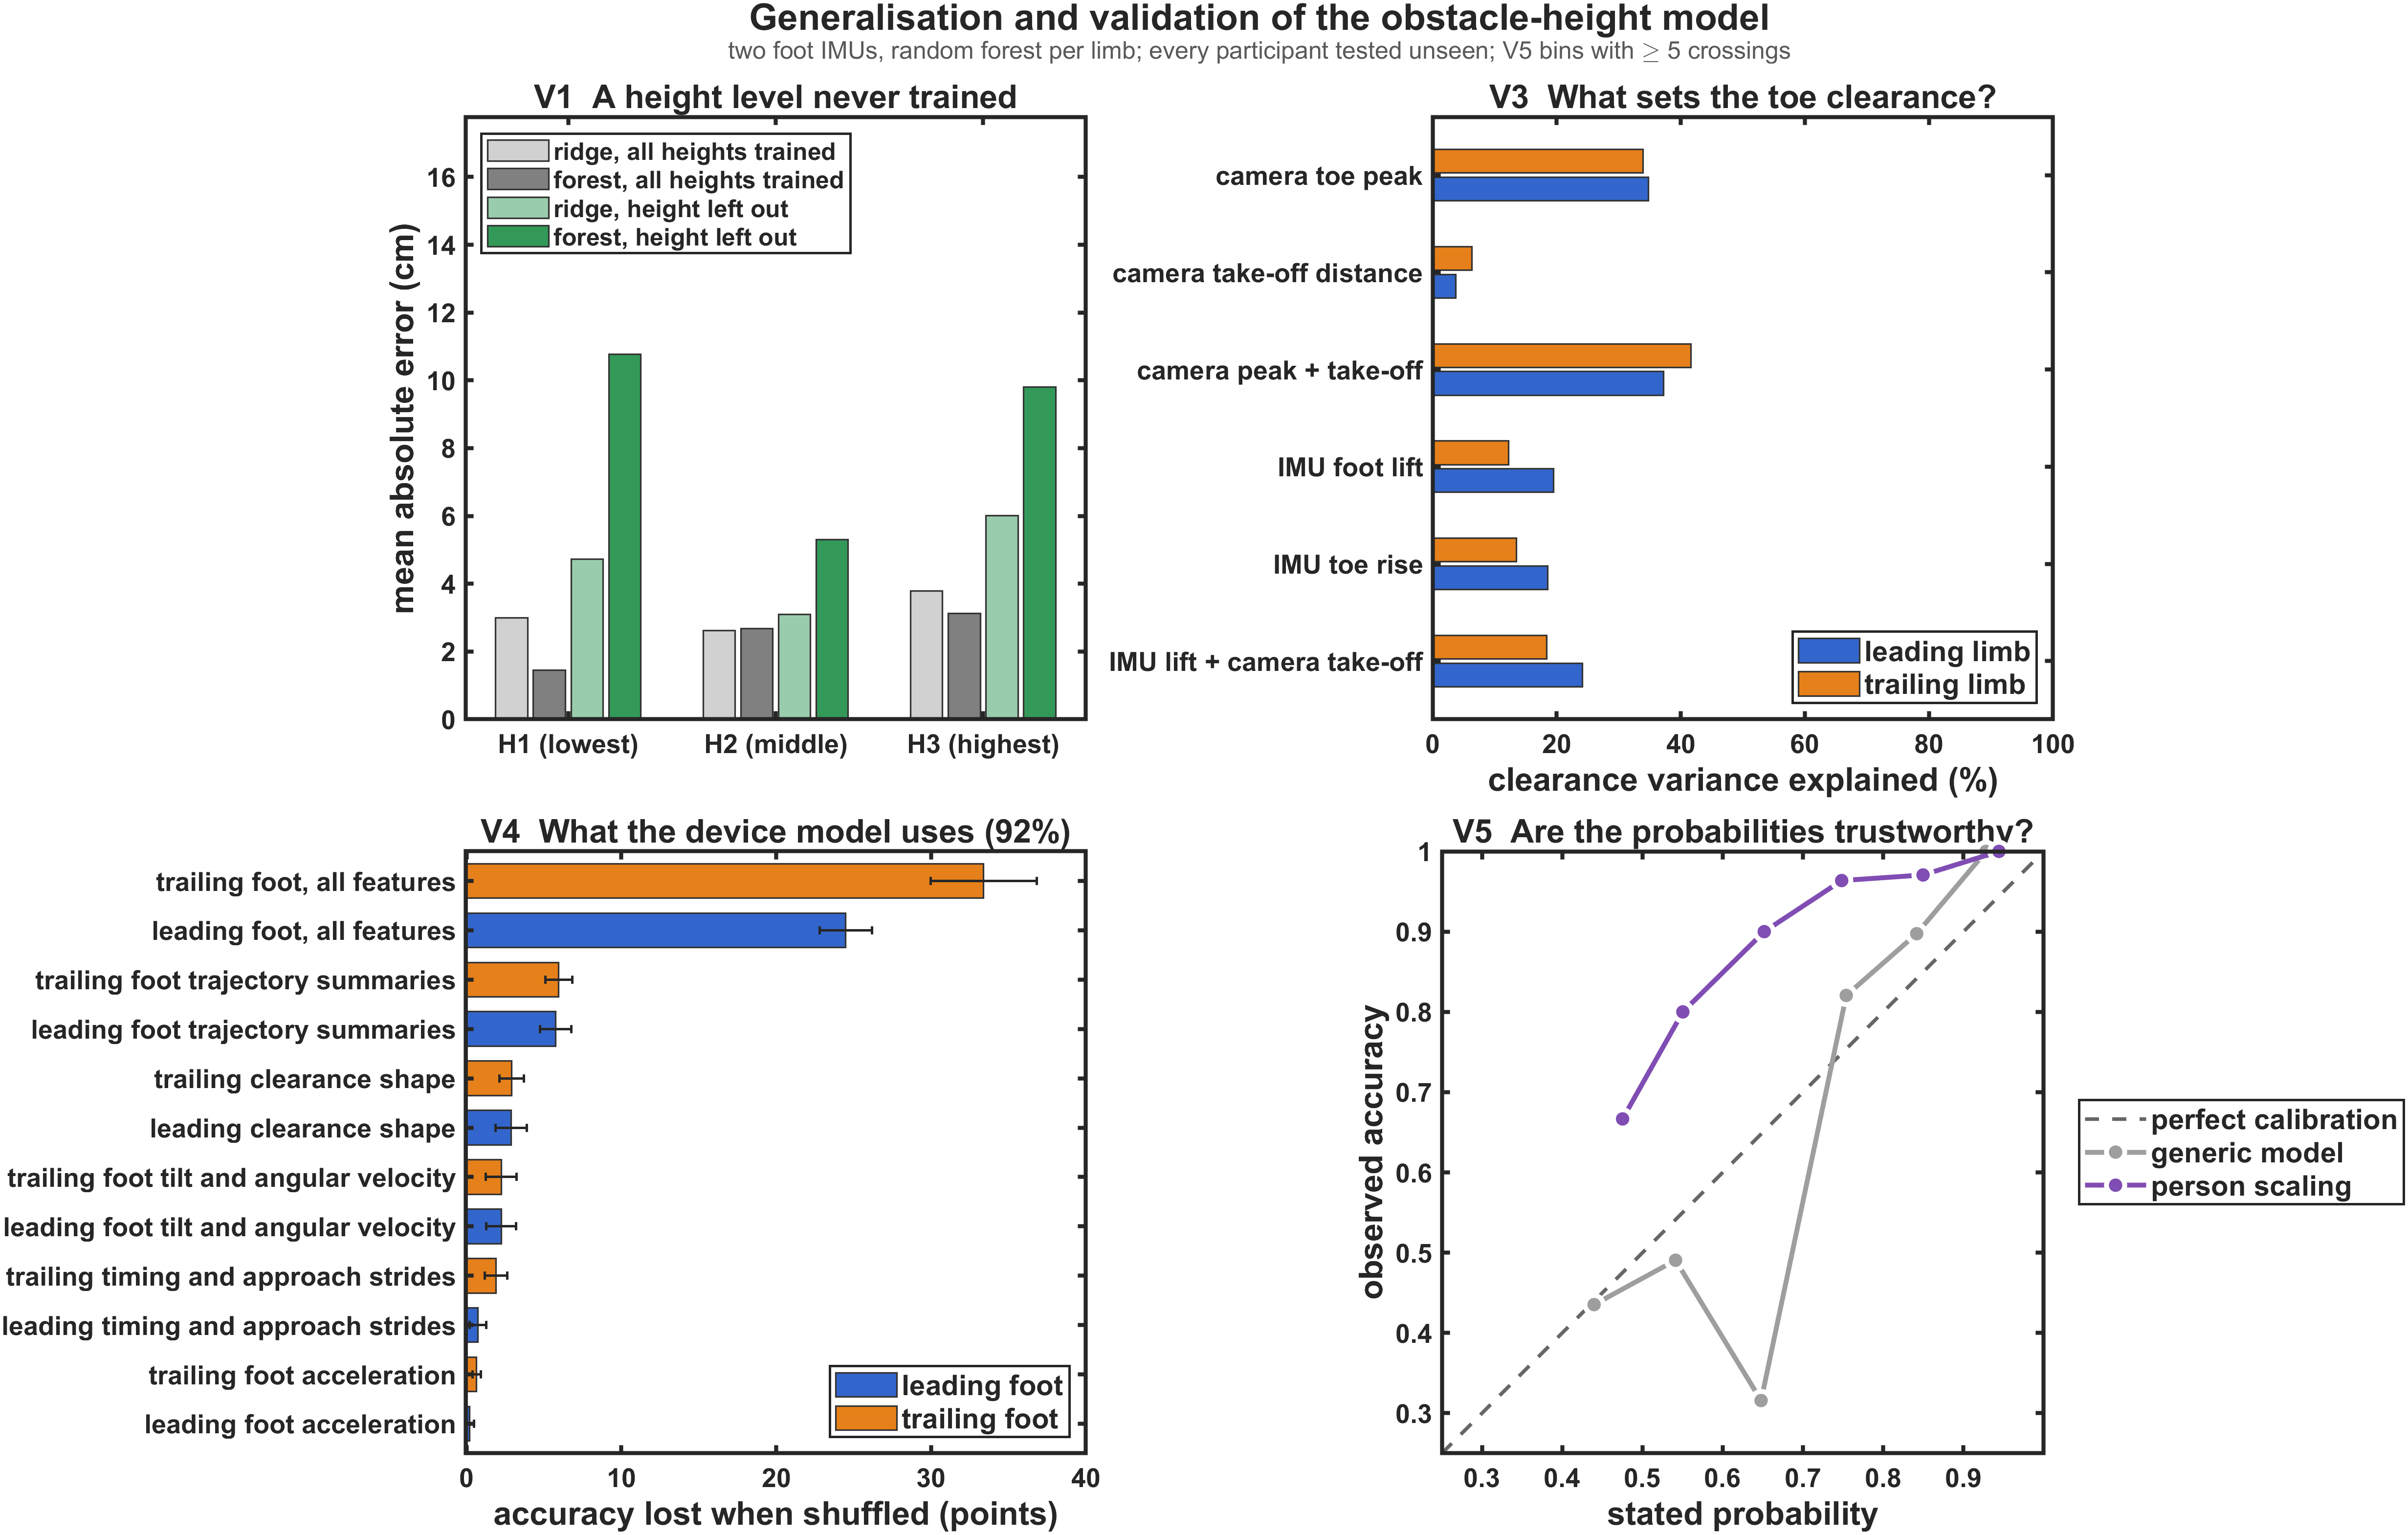
\includegraphics[width=\textwidth]{fig_validate.png}
\caption{Validation. V1: height error when a height level is missing from training (grey = trained on all heights, green = this
height left out; light = ridge, dark = forest). V3: what explains the crossing-to-crossing clearance (blue = leading, orange =
trailing limb). V4: accuracy lost when a feature group of the final model is shuffled (permutation importance). V5: reliability of
the stated probabilities (grey = generic, purple = person scaling, dashed = perfect calibration).}
\label{fig:validate}
\end{figure}

